\documentclass[11pt]{article}

\usepackage[
  paperwidth=8.5in,
  paperheight=36in,
  left=0.8in,
  right=0.8in,
  top=0.8in,
  bottom=1.5in,
]{geometry}
\usepackage{amsmath,amssymb}
\usepackage{graphicx}

\usepackage{tikz}
\usetikzlibrary{arrows.meta, positioning, fit, backgrounds, calc}


\usepackage[dvipsnames]{xcolor}
\usepackage{hyperref}
\definecolor{okabepink}{HTML}{CC79A7}
\definecolor{okabecyan}{HTML}{56B4E9}
\hypersetup{
  colorlinks = true,
  linkcolor  = black,
  citecolor  = black,
  urlcolor   = okabepink
}

\usepackage{listings}
\usepackage[most]{tcolorbox}
\tcbuselibrary{listings}

\definecolor{codebg}{RGB}{248,248,248}
\definecolor{codeframe}{RGB}{225,225,225}
\definecolor{codekw}{RGB}{120,70,160}
\definecolor{codecomment}{RGB}{100,120,100}
\definecolor{codestring}{RGB}{160,80,60}
\definecolor{codeattr}{RGB}{80,100,150}

\lstdefinelanguage{Rust}{
  sensitive=true,
  keywords={
    as,break,const,continue,crate,else,enum,extern,false,fn,for,if,impl,in,
    let,loop,match,mod,move,mut,pub,ref,return,self,Self,static,struct,
    super,trait,true,type,unsafe,use,where,while,async,await,dyn
  },
  keywordstyle=\color{codekw}\bfseries,
  comment=[l]{//},
  morecomment=[s]{/*}{*/},
  commentstyle=\color{codecomment}\itshape,
  morestring=[b]",
  stringstyle=\color{codestring},
  alsoletter={\#},
  moredelim=[s][\color{codeattr}]{\#[}{]},
}

\newtcblisting{rust}{
  listing engine=listings,
  listing only,
  colback=codebg,
  colframe=codeframe,
  boxrule=0.35pt,
  arc=2pt,
  left=10pt,
  right=10pt,
  top=9pt,
  bottom=9pt,
  width=\textwidth,
  before skip=0.8em,
  after skip=0.9em,
  listing options={
    language=Rust,
    basicstyle=\ttfamily\small,
    breaklines=true,
    columns=fullflexible,
    keepspaces=true,
    showstringspaces=false,
    tabsize=4,
    upquote=true
  }
}
\usepackage{enumitem}
\newlist{notelist}{itemize}{1}
\setlist[notelist]{
    label={--},
    leftmargin=2.0em,
    itemsep=0.2em,
    topsep=0.4em,
    parsep=0em
}

\title{
  Lean Design of Optimized Level-1 BLAS \\[0.25em]
  \large LAK Working Note \#2
}
\author{
  deval-d@stanford.edu 
}

\date{13 May 2026}

\begin{document}

\maketitle
\thispagestyle{empty} 

\begin{abstract}
The level-1 BLAS consists of $O(n)$ vector-vector routines with low arithmetic
intensity. Kernels are divided into two cases: routines without
loop-carried dependencies and routines with loop-carried dependencies. Direct
scalar loops are sufficient for the first case; the second case requires
independent accumulators with explicit manual SIMD to avoid serializing
the reduction. With contiguous vector views in \texttt{lak}, this gives a lean
implementation in which most kernels remain ordinary loops and only the
dependency-chain kernels contain manual SIMD instructions. \\[0.1em]

\noindent The compiler discussed is \texttt{rustc 1.94.0-nightly}. Other compilers may not have similar behavior.
\end{abstract}

\section{Dependency Chains} 

The level-1 BLAS routines operate on vectors. Examples include scaling a vector, adding one vector to another, 
copying data, taking a dot product, and computing vector norms. These routines all have $O(n)$ work, but they 
do not all present the same optimization problem to the compiler. 
The important distinction in this note is whether the natural scalar loop has
a \textit{loop-carried dependence}. A loop-carried dependence occurs when one
iteration of the loop needs a value produced by an earlier iteration. When no
such dependence exists, the iterations can be treated as independent pieces of
work. When such a dependence does exist, the loop looks sequential unless the
implementation rewrites it to expose more parallelism.

The \texttt{AXPY} routine is the simple case. It computes 
\begin{equation}
    y_i \leftarrow \alpha x_i + y_i. 
\end{equation}
Each index $i$ updates a different element of $y$. The calculation of $y_7$ does not depend on the 
result of the computation of $y_6$. This is the elementwise structure shown on the left of Figure \ref{fig:l1-dependencies}.
Once the compiler sees a clean loop over contiguous slices, the 
elementwise structure is explicit. On a modern target, LLVM can often turn that scalar loop into SIMD 
instructions \texttt{automatically}, even without the source code mentioning SIMD directly. 
This will be covered more in sections \ref{sec:axpy} and \ref{sec:dot}. 

The dot product has a different shape. It computes 
\begin{equation}
    x \cdot y = \sum_{i=0}^{n-1} x_i y_i . 
\end{equation}
A direct scalar implementation naturally introduces a running sum: 

\begin{rust} 
pub fn dot<T>( 
    x: VecRef<'_, T>, 
    y: VecRef<'_, T>, 
) -> T 
where 
    T: Default 
        + Copy 
        + Fma 
        + Mul<Output=T> 
        + Add<Output=T>, 
{
    // ensures buffers have equal length
    assert_n_eq!(x, y); 

    // access stored &[T] buffer; 
    let xdata = x.as_slice(); 
    let ydata = y.as_slice(); 

    // running sum 
    let mut sum = T::default(); 
    for (&xi, &yi) in xdata.iter().zip(ydata.iter()) { 
        // dependency chain 
        // sum += xi * yi
        sum = xi.fma(yi, sum); 
    }

    sum
}
\end{rust} 

The inner loop does not merely compute an independent output for each index. Instead, 
each iteration reads the current value of \texttt{sum} and produces the next value of 
\texttt{sum}. The value produced at iteration $i$ is therefore an input to iteration $i+1$. This 
is the dependency chain shown on the right side of Figure \ref{fig:l1-dependencies}. This does not mean the dot product is impossible to vectorize. The products $x_i y_i$ are independent. 
What is serial in the naive loop is the single accumulated \texttt{sum} state. To use SIMD well, 
the implementation must change the \textit{shape} of the computation: instead of one running sum, 
it uses several independent \textit{partial} sums and combines them at the end, outside of the inner loop. 
This rewrite is the main subject of section \ref{sec:dot}. 

\begin{figure}[h]
\centering
\begin{tikzpicture}[
    scale=1.12,
    every node/.style={transform shape},
    font=\small,
    cell/.style={
        draw=black,
        rectangle,
        minimum width=0.34cm,
        minimum height=0.34cm,
        inner sep=0pt,
        line width=0.4pt
    },
    state/.style={
        draw=black,
        rectangle,
        minimum width=0.50cm,
        minimum height=0.36cm,
        inner sep=0pt,
        line width=0.4pt
    },
    op/.style={
        draw=black,
        circle,
        minimum size=0.26cm,
        inner sep=0pt,
        line width=0.4pt
    },
    arrow/.style={
        -{Latex[length=1.35mm,width=1.05mm]},
        line width=0.4pt,
        draw=black
    },
    dep/.style={
        -{Latex[length=1.45mm,width=1.15mm]},
        line width=0.55pt,
        draw=black
    },
    title/.style={
        font=\small,
        inner sep=1pt
    },
    label/.style={
        font=\footnotesize,
        inner sep=1pt
    }
]


\begin{scope}
    \foreach \i in {0,...,5} {
        \node[cell] (x\i) at ({0.58*\i},1.35) {};
        \node[cell] (y\i) at ({0.58*\i},0.55) {};
        \node[op]   (f\i) at ({0.58*\i},-0.05) {};
        \node[cell] (z\i) at ({0.58*\i},-0.65) {};

        \draw[bareline] (x\i.south) -- (y\i.north);
        \draw[arrow]   (y\i.south) -- (f\i.north);
        \draw[arrow] (f\i.south) -- (z\i.north);
    }

    \node[title] at ($(x0)!0.5!(x5)+(0,0.58)$) {pure elementwise};

    \node[label, left=0.28cm of x0] {$x$};
    \node[label, left=0.28cm of y0] {$y$};
    \node[label, left=0.28cm of z0] {$y'$};
\end{scope}

\begin{scope}[xshift=6.15cm]
    \foreach \i/\x in {0/0,1/1.05,2/2.10,3/3.15} {
        \node[cell]  (u\i) at (\x,1.35) {};
        \node[op]    (g\i) at (\x,0.35) {};
        \node[state] (s\i) at (\x,-0.65) {};

        \draw[arrow] (u\i.south) -- (g\i.north);
        \draw[arrow] (g\i.south) -- (s\i.north);
    }

    \draw[dep]
        (s0.east) .. controls +(0.38,0.05) and +(-0.38,-0.05) .. (g1.west);
    \draw[dep]
        (s1.east) .. controls +(0.38,0.05) and +(-0.38,-0.05) .. (g2.west);
    \draw[dep]
        (s2.east) .. controls +(0.38,0.05) and +(-0.38,-0.05) .. (g3.west);

    \node[title] at ($(u0)!0.5!(u3)+(0,0.58)$) {dependency-chain};

    \node[label, left=0.28cm of u0] {$u$};
    \node[label, left=0.28cm of s0] {$s$};

\end{scope}

\end{tikzpicture}

\caption{Classification of the level-1 kernels. Elementwise routines expose independent work directly. Dependency-chain routines carry state between iterations, hiding the available parallelism behind a scalar recurrence.}
\label{fig:l1-dependencies}
\end{figure}

This gives the organizing principle for the rest of the note. For elementwise kernels, the main 
job is to expose a clean contiguous loop and let the compiler automatically emit SIMD. Even if the 
compiler-generated SIMD code is minimally unrolled, the very low arithmetic intensity of the level-1 BLAS 
allows such code to still be roughly optimal. For reduction kernels, the main job is to re-design the 
implementation to remove scalar recurrence from the hot loop via introducing independent accumulators. 

\section{\texttt{AXPY}} \label{sec:axpy}

\begin{figure}[h]
\centering
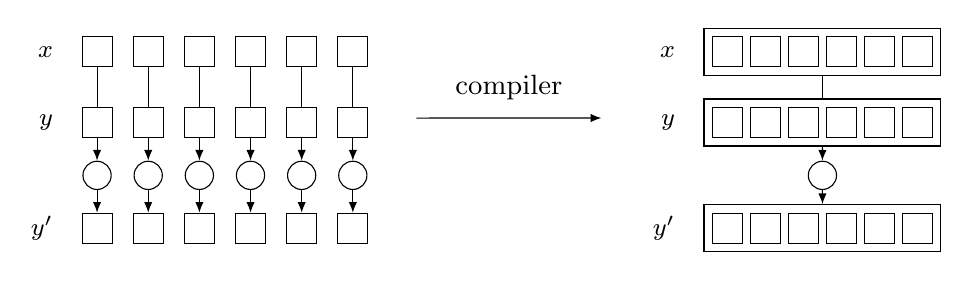
\begin{tikzpicture}[
    scale=1.12,
    every node/.style={transform shape},
    font=\small,
    cell/.style={
        draw=black,
        rectangle,
        minimum width=0.34cm,
        minimum height=0.34cm,
        inner sep=0pt,
        line width=0.4pt
    },
    op/.style={
        draw=black,
        circle,
        minimum size=0.32cm,
        inner sep=0pt,
        line width=0.4pt
    },
    arrow/.style={
        -{Latex[length=1.35mm,width=1.05mm]},
        line width=0.4pt,
        draw=black
    },
    bareline/.style={
        line width=0.4pt,
        draw=black
    },
    group/.style={
        draw=black,
        rectangle,
        inner sep=0.10cm,
        line width=0.5pt
    },
    label/.style={
        font=\footnotesize,
        inner sep=1pt
    }
]

% ============================================================
% Left: scalar elementwise lanes
% ============================================================

\begin{scope}[local bounding box=scalar]
    \foreach \i in {0,...,5} {
        \node[cell] (x\i) at ({0.58*\i}, 1.35) {};
        \node[cell] (y\i) at ({0.58*\i}, 0.55) {};
        \node[op]   (f\i) at ({0.58*\i},-0.05) {};
        \node[cell] (z\i) at ({0.58*\i},-0.65) {};

        \draw[bareline] (x\i.south) -- (y\i.north);
        \draw[arrow]   (y\i.south) -- (f\i.north);
        \draw[arrow]   (f\i.south) -- (z\i.north);
    }

    \node[label, left=0.28cm of x0] {$x$};
    \node[label, left=0.28cm of y0] {$y$};
    \node[label, left=0.28cm of z0] {$y'$};
\end{scope}

% ============================================================
% Right: SIMD packed lane
% ============================================================

\begin{scope}[xshift=7.15cm, local bounding box=simd]
    \foreach \i in {0,...,5} {
        \node[cell] (vx\i) at ({0.43*\i}, 1.35) {};
        \node[cell] (vy\i) at ({0.43*\i}, 0.55) {};
        \node[cell] (vz\i) at ({0.43*\i},-0.65) {};
    }

    \node[group, fit=(vx0)(vx1)(vx2)(vx3)(vx4)(vx5)] (gx) {};
    \node[group, fit=(vy0)(vy1)(vy2)(vy3)(vy4)(vy5)] (gy) {};
    \node[group, fit=(vz0)(vz1)(vz2)(vz3)(vz4)(vz5)] (gz) {};

    \node[op] (vf) at ({0.43*2.5}, -0.05) {};

    % Connect only between outer SIMD boxes and the circle.
    \draw[bareline] (gx.south) -- (gy.north);
    \draw[arrow]   (gy.south) -- (vf.north);
    \draw[arrow]   (vf.south) -- (gz.north);

    \node[label, left=0.28cm of gx] {$x$};
    \node[label, left=0.28cm of gy] {$y$};
    \node[label, left=0.28cm of gz] {$y'$};
\end{scope}

% ============================================================
% Compiler arrow
% ============================================================

\coordinate (L) at ($(scalar.east)+(0.55,0.25)$);
\coordinate (R) at ($(simd.west)+(-0.55,0.25)$);

\draw[arrow] (L) -- (R);
\node[above=0.08cm] at ($(L)!0.5!(R)$) {compiler};

\end{tikzpicture}

\caption{Independent elementwise iterations are automatically widened into a single SIMD operation.}
\label{fig:auto-simd-elementwise}
\end{figure}

\section{\texttt{DOT}} \label{sec:dot}

\begin{figure}[h]
\centering
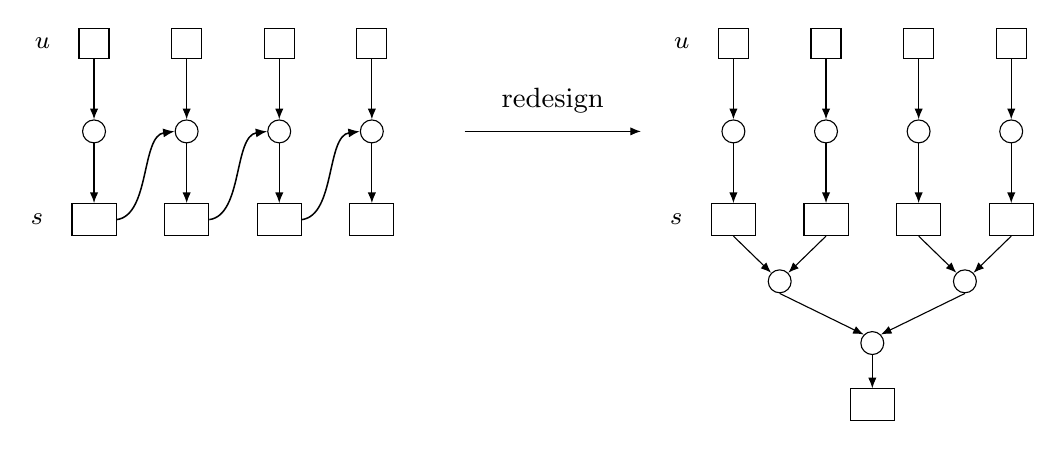
\begin{tikzpicture}[
    scale=1.12,
    every node/.style={transform shape},
    font=\small,
    cell/.style={
        draw=black,
        rectangle,
        minimum width=0.34cm,
        minimum height=0.34cm,
        inner sep=0pt,
        line width=0.4pt
    },
    state/.style={
        draw=black,
        rectangle,
        minimum width=0.50cm,
        minimum height=0.36cm,
        inner sep=0pt,
        line width=0.4pt
    },
    op/.style={
        draw=black,
        circle,
        minimum size=0.26cm,
        inner sep=0pt,
        line width=0.4pt
    },
    arrow/.style={
        -{Latex[length=1.35mm,width=1.05mm]},
        line width=0.4pt,
        draw=black
    },
    dep/.style={
        -{Latex[length=1.45mm,width=1.15mm]},
        line width=0.55pt,
        draw=black
    },
    label/.style={
        font=\footnotesize,
        inner sep=1pt
    }
]

% ============================================================
% Left: running accumulator dependency chain
% ============================================================

\begin{scope}
    \foreach \i/\x in {0/0,1/1.05,2/2.10,3/3.15} {
        \node[cell]  (u\i) at (\x,1.35) {};
        \node[op]    (g\i) at (\x,0.35) {};
        \node[state] (s\i) at (\x,-0.65) {};

        \draw[arrow] (u\i.south) -- (g\i.north);
        \draw[arrow] (g\i.south) -- (s\i.north);
    }

    \draw[dep]
        (s0.east) .. controls +(0.38,0.05) and +(-0.38,-0.05) .. (g1.west);
    \draw[dep]
        (s1.east) .. controls +(0.38,0.05) and +(-0.38,-0.05) .. (g2.west);
    \draw[dep]
        (s2.east) .. controls +(0.38,0.05) and +(-0.38,-0.05) .. (g3.west);

    \node[label, left=0.28cm of u0] {$u$};
    \node[label, left=0.28cm of s0] {$s$};
\end{scope}

% ============================================================
% Right: independent accumulators, reduction afterward
% ============================================================

\begin{scope}[xshift=7.25cm]
    \foreach \i/\x in {0/0,1/1.05,2/2.10,3/3.15} {
        \node[cell]  (v\i) at (\x,1.35) {};
        \node[op]    (h\i) at (\x,0.35) {};
        \node[state] (a\i) at (\x,-0.65) {};

        \draw[arrow] (v\i.south) -- (h\i.north);
        \draw[arrow] (h\i.south) -- (a\i.north);
    }

    \node[op] (r01) at (0.525,-1.35) {};
    \node[op] (r23) at (2.625,-1.35) {};
    \node[op] (r)   at (1.575,-2.05) {};
    \node[state] (out) at (1.575,-2.75) {};

    \draw[arrow] (a0.south) -- (r01.north west);
    \draw[arrow] (a1.south) -- (r01.north east);

    \draw[arrow] (a2.south) -- (r23.north west);
    \draw[arrow] (a3.south) -- (r23.north east);

    \draw[arrow] (r01.south) -- (r.north west);
    \draw[arrow] (r23.south) -- (r.north east);

    \draw[arrow] (r.south) -- (out.north);

    \node[label, left=0.28cm of v0] {$u$};
    \node[label, left=0.28cm of a0] {$s$};
\end{scope}

% ============================================================
% Redesign arrow, explicitly horizontal and longer
% ============================================================

% ============================================================
% Redesign arrow, matched to AXPY compiler-arrow length
% ============================================================

\coordinate (M) at ($(g3.east)!0.5!(h0.west)$);

\draw[arrow] ($(M)+(-1,0)$) -- ($(M)+(1,0)$);
\node[above=0.08cm] at (M) {redesign};
\end{tikzpicture}

\caption{A running accumulator creates a loop-carried dependency. Splitting the work across independent accumulators exposes parallelism inside the loop; the partial sums are reduced afterward.}
\label{fig:sdot-redesign}
\end{figure}

\end{document}
